\chapter{Literature review}
\label{chap:Literature review}
This chapter firstly reviews the spatial features of human poses and the temporal features involved in the video data set, as well as the classic methods used to processing these features in section \ref{sec:Data features and classic methods}.
Then, section \ref{sec:Online exam security system} surveys the previous research and technical applications on the online exam security system, the application scenarios of this project.
Before studying the related research using deep learning, section \ref{sec:Deep models detail} studies the details of several deep models comprehensively.
After understanding the related concepts and basic operations and backbones of the deep models, section \ref{sec:Related works using deep models} reviews numerous human activity recognition related works based on deep learning models.
Finally, section \ref{sec:Mobile device optimisation} mentions some methods of optimising models so that it can run on devices with limited computing power such as mobile phones.
\section{Data features and classic methods}
\label{sec:Data features and classic methods}
% 2 pages
To study the feasibility of this project, and to utilise deep learning methods to classify actions from sequential imagery features, videos containing pose-based data, comprehensively reviewing the previous research on data features and feature engineering methods is beneficial to the design of deep models.

%Characteristics of video-based data set
\begin{minipage}[ht]{.48\textwidth}
    \begin{figure}[H]
        \centering
        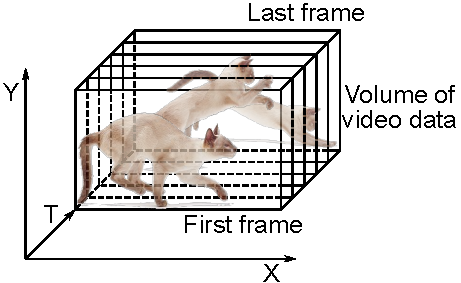
\includegraphics[scale=0.9]{literature/imgs/1-video-volume.pdf}
        \caption{Cubic volume of video data}
        \label{fig:1-video-volume}
    \end{figure}
\end{minipage}
\begin{minipage}[ht]{.5\textwidth}
    \begin{figure}[H]
        \centering
        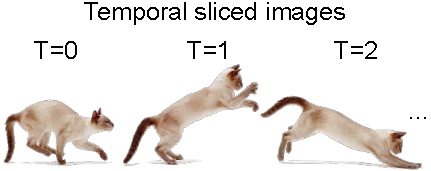
\includegraphics{literature/imgs/2-video-slice.pdf}
        \caption{Slicing the video cube parallel to the X-Y axis}
        \label{fig:2-video-slice}
    \end{figure}
\end{minipage}

Video is composed of a sequence of image data and synchronised audio arranged in the timeline. 
If the audio data beyond the scope of this study is ignored, the 2D images can be stacked along the time axis to form a 3D cube representing the video. Figure \ref{fig:1-video-volume} illustrates an intuitive representation proposed by \citet{fels1999interactive}, which highlights the spatial and temporal characteristics for all videos.
Further, figure \ref{fig:1-video-volume} shows that regular video frames produced by slicing the video cube parallel to the $X-Y$ axis so that computer vision algorithms or depth models for visual tasks can be applied.
As a result, video can be simplified into a series of images to enable applying image processing technology.

%Characteristics of human pose-based features
In each static image containing human pose-based features, what features can be used for posture analysis to classify each image? 
\citet{thrasher2011mood} model the features worthy of attention in human upper body poses and then conduct a pose-based study on mood recognition by analysing and rating the postures of the head, shoulders, trunk, arms in video data.
The dataset in their research is closely analogous to the dataset in this research because both datasets comprise human facial expressions and upper body poses.

%Link pose-based and video-based features
From posture analysis in a single image to human action recognition in sequential images, it combines pose-based features and video-based data.
For example, \citet{yao2016spatio} propose a paper on spatio-temporal feature extraction with a variety of application scenarios in automatic human activity recognition, such as video information retrieval, intelligent surveillance, and human-computer interaction.
In future research, they point out that deep learning can be a powerful tool for processing these spatio-temporal features and thus will enable the low-level engineered features to fuse with a deep learning framework.

Before deep learning methods are prevalent in the computer vision field, some previous studies have built data sets for the human action recognition task and have conducted studies with classic machine learning methods.

Support vector machines (SVM), a well-known classic machine learning method, has been applied in many researches related to human action recognition.
For example, \citet{schuldt2004recognizing} extract local events such as size, frequency and velocity of moving patterns from videos and create a new video database, KTH dataset \footnote{Recognition of human actions: \url{https://www.csc.kth.se/cvap/actions/}}, to evaluate the proposed human actions classification with the SVM method.
Using the SVM method, they carefully model the data representation based on local spatio-temporal features and select appropriate features, kernel tricks, and hyperparameters to obtain the desired results.
%\citet{gorelick2007actions}

Further, \citet{marszalek2009actions} believes that human actions are highly correlated with background scenes, which means the context of the scene can help identify human actions in videos.
They creatively use movie scripts and movie videos, Hollywood-2 dataset \footnote{Human Actions and Scenes Dataset: \url{https://www.di.ens.fr/~laptev/actions/hollywood2/}}, to train ``a joint scene-action SVM-based classifier'' with script-to-video alignment.
They explained in detail how to get aligned target actions and target scenes from movies and also used $\mathcal{X}^2$ kernel function in SVM classifier, similar to the research by \citet{schuldt2004recognizing}.

\citet{Soomro2014} % 2 pages
\section{Online exam security system}
\label{sec:Online exam security system}
% 1 pages
In order to learn about the background of the security system of remote exams and propose a new system that better adapts to the status quo, this research reviews the previous research on the security system of online exams in this section.

Before the COVID-19 pandemic, the technology of paperless testing through computer systems has been widely used. For example, TOEFL iBT (Internet-based test) has gradually replaced the PBT (paper-based test) by using the Internet and computers for paperless exams from late 2005.
Another example is specific exams that are impossible to be sat on paper, such as programming competitions or exams requiring running compilers.
Although all these exams were in the form of using computers and the Internet, students were required to congregate in testing centers.

% Authentication
As a result, most of the previous research in this field assumes that the exam can still be organised in test centres, so the research direction of exam security focusing on biometric authentication.
For example, \citet{traore2017ensuring} propose a multi-modal biometric authentication framework, including face biometric and dynamic biometric from computer input devices, such as mouse and keyboard.
The purpose of biometric authentication is to prevent imposters in the exam, and the invigilators of the test centre should detect other cheating in time.

Nowadays, the pandemic segregates students at home for remote exams, invalidating the previous assumption.
There are still some studies proposing new solutions for biometric authentication in exams. 
In Japan, \citet{Akiko202144107} propose a new continuous biometric authentication method based on hand image features, which can prevent cheating, especially impersonation due to lack of invigilation. 
They use a mirror and a wide-angle lens to capture the images of students' hands when they take the exam and obtain the contour features of the hands through image processing.
However, any biometric authentication cannot prevent cheating by the students per se, such as using mobile phones to search online or seeking help from others.

In 2020, \citet{garg2020convolutional} point out that many security issues still exist in online exams, and propose a system based on Haar Cascade Classifier and Convolutional Neural Network to detect, track, tag, and identify the student's face.
Although this system innovatively uses deep learning models, only using facial features and constraints in the design is not comprehensive compared to action recognition.
And another disadvantage is focusing on facial features may cause contention in privacy risks mentioned in the research ethics section \ref{sec:Research ethics}.
For example, students can still cheat with mobile phones during online exams even with the facial-based security system enabled.

% confirm originality
After investigating many previous studies on online exam security systems, it is concluded that most of the research is limited to biometrics authentication, and there is no readily available security system that equips a deep-learning-based human action recognition model.
As a result, this research originally applied the human action recognition technique to the online exam security system.
 % 1.5 pages
\section{Deep models details}
\label{sec:Deep models details}
% 4 pages
\subsection{Convolutional neural network}
% 3DCNN
\subsection{Recurrent neural network}
% et optimus
\subsection{Attention and transformer}

\subsection{State-of-the-art models} % 4 pages
\section{Related works using deep models}
\label{sec:Related works using deep models}
% 4 pages
% review 0.5 page
\subsection{Human action recognition overview}
\citet{wu2017recent}

\citet{chen2020monocular}
 % 1 page

% 3DCNN %% Video related 1.5 page
\subsection{3D-CNN and RNN based methods}
\label{subsec: 3D-CNN and RNN based methods}
The standard two-dimensional convolution uses a two-dimensional kernel filter on each channel, and only two-dimensional features can be extracted.
\citet{tran2015learning} reviewed many previous 3-dimensional convolutional networks (3D-CNN) and highlighted relevant applications on spatiotemporal features in video dataset.
As shown in Figure \ref{fig:2-2dcnn-3dcnn}, 2D convolutional kernel filters are expanded to 3D and allow them running on multiple channels simultaneously.
3D-CNN is widely used in tasks that process multiple images at the same time, such as medical computed tomography (CT) scan data and video data.

\begin{figure}[!ht]
    \centering
    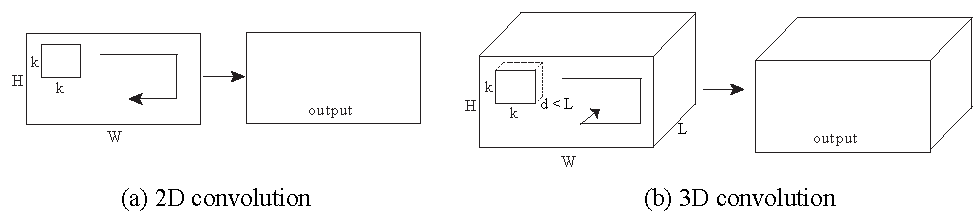
\includegraphics[width=\textwidth]{literature/imgs/2-2dcnn-3dcnn.pdf}
    \caption{2D convolution and 3D convolution \cite{tran2015learning}}
    \label{fig:2-2dcnn-3dcnn}
\end{figure}

The difference between the proposed 3D convolution and the multi-channel 2D convolution is that the 3D convolution uses weight-sharing kernel filters, while the multi-channel 2D convolutional kernel filters have different weights for each channel and ignore adjacent channels in computation.

Back to 2011, \citet{baccouche2011sequential} firstly applied a composed architecture of 3D convolution and RNN to the human action recognition task.
In this work, 3D convolution is firstly used for learning spatiotemporal features automatically, followed by an RNN `` to classify each sequence considering the temporal evolution of the learned features for each timestep'', said by \citet{baccouche2011sequential}.
The researchers also spotted the performance drawback of the RNN and will investigate the possibility of using a single-step model in future work.

One year after, \citet{ji20123d} proposed a human action recognition model composed purely of convolutional operations. %, as shown in Figure \ref{fig:ext-2-3dcnn-har}.
The premature network design is shallow and does not use residual connections, which are very similar in architecture to LeNet, consisting of multiple convolutional layers and pooling layers. In addition, they add some designed features (optical flow fields in many directions) to input, which is not an end-to-end trainable network.

% \begin{figure}[!ht]
%     \centering
%     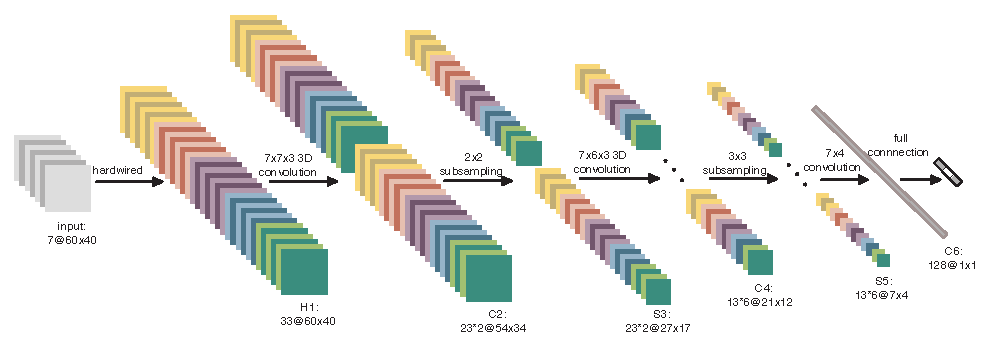
\includegraphics[width=\textwidth]{literature/imgs/ext-2-3dcnn-har.pdf}
%     \caption{A 3D-CNN model for human action recognition \cite{ji20123d}}
%     \label{fig:ext-2-3dcnn-har}
% \end{figure}

After several years of development, \citet{tran2015learning} proposed model Convolutional 3D (C3D) that achieved the state-of-the-art in video tasks in 2015.
This model does not involve the input of additional handcrafted features at all, but it also exposes some weaknesses of the 3D convolution.
For example, 3D-CNN cannot use pre-trained results from 2D images, such as ImageNet.
Also, the network has too many parameters, which is prone to over-fitting in the case of using an insufficient amount of video training data.

To overcome the weaknesses of using CNN or RNN individually, \citet{simonyan2014twostream} proposed a Two-Stream network.
The network consists of a spatial flow focused on each image frame and a temporal flow focused on the calculated optical flow.
Based on the idea of using the Two-Stream network, \citet{feichtenhofer2016convolutional} pointed out that the fusion process in the last Softmax layer caused losses and 3D convolution can perfectly fuse the spatiotemporal information in the convolutional layers.

In 2018, \citet{carreira2018quo} summarised the previous research on different methods used in the field of action recognition, which is also discussed in this subsection, namely ConvNet+LSTM (CNN+RNN), 3D ConvNets (3D-CNN) and Two-Stream network.
Based on these previous ideas, Inflated Two-Stream 3D ConvNets (I3D) is proposed and achieved good results on both HMDB-51 and UCF-101 data sets. % 1 page

\subsection{Transformer-based Neural Networks}

\citet{sun2019learning}

\citet{neimark2021video}

\begin{figure}[!ht]
    \centering
    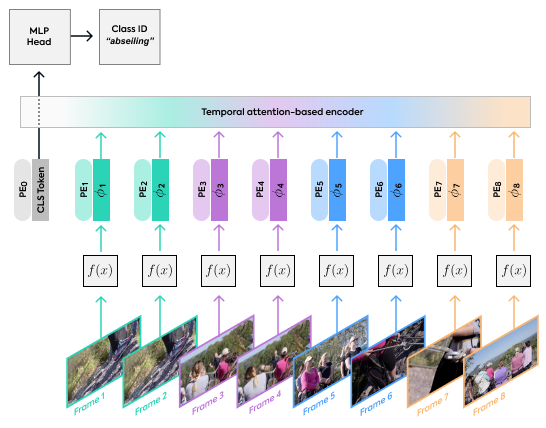
\includegraphics[width=.7\textwidth]{literature/imgs/ext-vtn.png}
    \caption{Video Transformer Network architecture \cite{neimark2021video}}
    \label{fig:ext-vtn}
\end{figure} % 2 page % 5 pages
\section{Mobile device optimisation}
\label{sec:Mobile device optimisation}
% 2 pages % 2 pages